\chapter{OpenDQ results}
\label{sec:07-results}
This chapter presents the results that can be obtained using the OpenDQ project using FSA (Frame Slotted ALOHA) and DQ (Distributed Queuing) as MAC protocols for the data transmission phase. In order to reproduce the experiments it is necessary to have 11 OpenMote-CC2538 boards, 1 OpenBase board and 10 OpenBattery boards, as well as 20 AAA batteries. To reproduce the experiments program 1 OpenMote-CC2538 as Gateway and 10 OpenMote-CC2538 as Node. The Gateway device needs to be connected to the computer using the OpenBase, whereas the 10 Node devices need to be connected to an OpenBattery board. Once programmed, execute the OpenDQ application and follow the experiments and results described in the next sections.

%%
% Frame-Slotted ALOHA
%%
\section{Frame-Slotted ALOHA}
The performance of FSA depends on the number of slots per frame ($k$) and the number of nodes that are present in the network ($n$). A number of slots per frame smaller than the number of nodes present in the network ($k<n$) will lead to a large number of collisions, whereas a number of slots per frame larger than the number of nodes present in the network ($k>n$) will lead to a large number of empty slots per frame. The theoretical optimal performance is achieved when the number of slots per frame is the same as the number of nodes in the network ($k=n$), which translates into a success probability of $36.8\%$ ($1/e$).

This results, however, assume that the physical layer is ideal, e.g., all nodes are received with the same power at the gateway. Unfortunately, the reality is that even small differences in the power with which the network coordinator receives each node present in the network, i.e., caused by differences in impedance matching in the antenna front end or by physical distance of the nodes with respect to the gateway, will have an impact on FSA performance. Such impact is translated into nodes that are \textit{closer} to the gateway have a higher probability of transmitting a successful packet, i.e., they capture the channel. This situation creates an unfairness in the network since nodes that are farther have a lower probability of transmitting a successful packet and, thus, have to spend more energy to transmit their packets. Since nodes are battery operated devices, this creates a situation in which the battery of nodes that are at the edge will be depleted faster than nodes that are at the core.

In the following paragraphs the performance of FSA is demonstrated with various number of slots per frame and various number of contending nodes present in each configuration. The first experiment is with one slot per frame and only one node in the network ($k=1$, $n=1$). As it can be seen in Figure~\ref{fig:07-fsa-k1n1}, the success probability of the node is $100\%$ and the collision and empty probability is $0\%$. This is because the node does not contend with any other node to access the single slot that is available in each frame.

% FSA results with k=n=1
\begin{figure}[!ht]
    \centering
	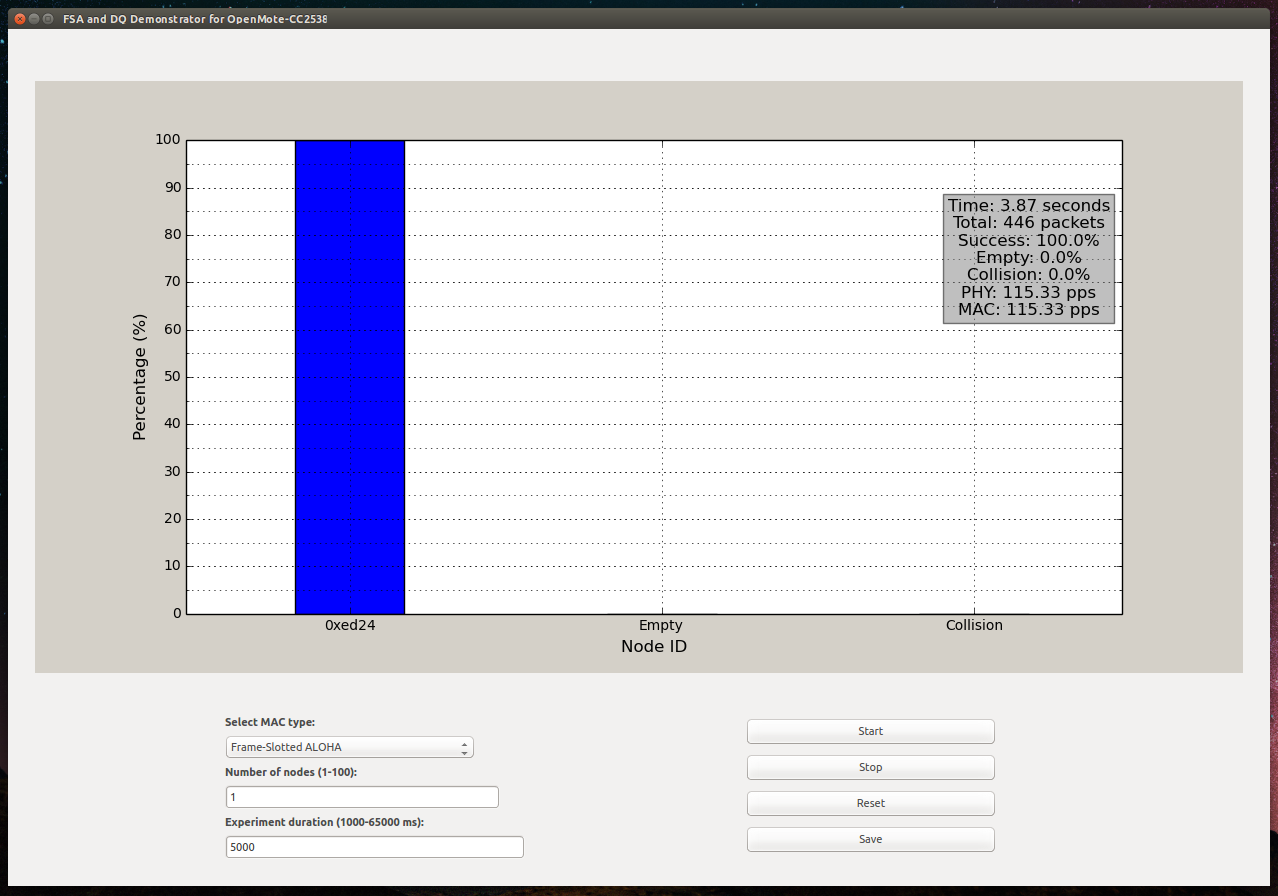
\includegraphics[width=0.75\linewidth]{07-fsa-k1n1}
    \caption{FSA results with $k=1$, $n=1$.}
    \label{fig:07-fsa-k1n1}
\end{figure}

The second experiment is with two slots per frame and five nodes in the network ($k=2$, $n=5$). In such configuration the success probability of each node should be around $3\%$ \footnote{In FSA the probability of a device successfully transmitting its data packet in a given frame with $m$ slots and $n$ contending nodes, assuming that there are neither transmission errors nor capture effect, can be calculated as $p_{s} = (\frac{1}{m}) \cdot (1 - \frac{1}{m})^{(n - 1)}$.} and the overall success probability should be around $15\%$. However, as depicted in Figure~\ref{fig:07-fsa-k2n5}, it is possible to observe that the success probability is not the same for each node, i.e., node $0x7faf$ is around $20\%$ whereas node $0xeca4$ is around $5\%$. This is due to the capture effect, as explained earlier, which also affects the overall success probability in a positive way, i.e., it is around $51.59\%$ instead of the theoretical $15\%$.

% FSA results with k=2, n=5
\begin{figure}[!ht]
    \centering
	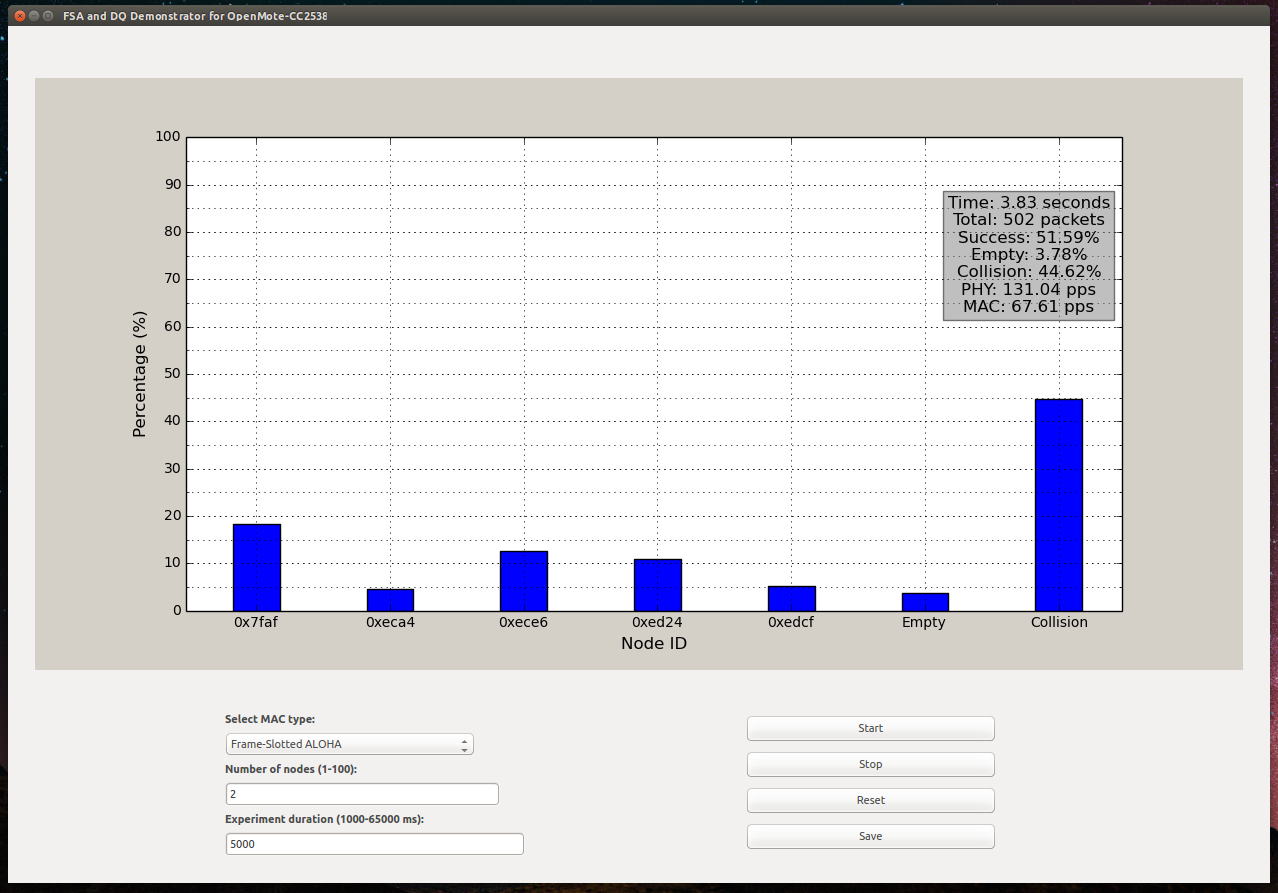
\includegraphics[width=0.75\linewidth]{07-fsa-k2n5}
    \caption{FSA results with $k=2$, $n=5$.}
    \label{fig:07-fsa-k2n5}
\end{figure}

In the third experiment the number of slots per frame is the same but the number of contending nodes increases to ten ($k=2$, $n=10$). According to the formula presented earlier, under such conditions the success probability of each node should be around $0.1\%$ and the overall success probability should be around $1\%$. However, as depicted in Figure~\ref{fig:07-fsa-k2n10}, the obtained overall success probability is above the theoretical value ($12.15\%$) and it is also possible to observe that a given node ($xece6$) is still capable to transmit its data packets with a success probability higher than the remaining nodes ($~5\%$). As explained earlier, such outcome is due to the capture effect.

% FSA results with k=2, n=10
\begin{figure}[!ht]
    \centering
	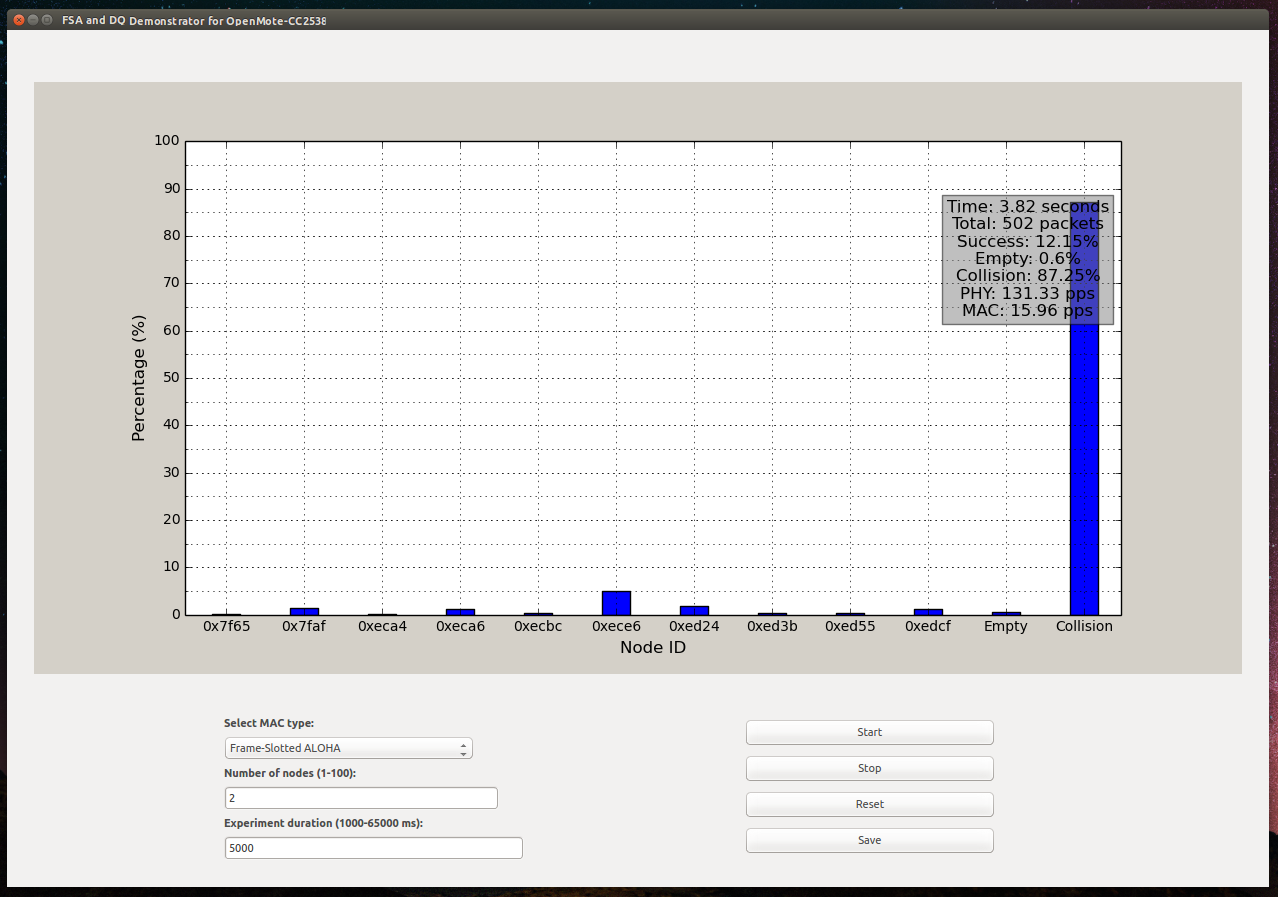
\includegraphics[width=0.75\linewidth]{07-fsa-k2n10}
    \caption{FSA results with $k=2$, $n=10$.}
    \label{fig:07-fsa-k2n10}
\end{figure}

In the fourth experiment, the number of slots per frame is larger than the number of contending nodes ($k=5$, $n=2$). According to the formula presented earlier, under such conditions the success probability of each individual node should be $16\%$ and the overall success probability should be $32\%$. As depicted in Figure~\ref{fig:07-fsa-k5n2}, the individual node success probability is around $16\%$ and the overall success probability is $32.78\%$. Such results are in accordance with the theoretical results because, given the low probability of two nods selecting the same slot, the capture effect does not play a significant role in the overall results.

% FSA results with k=5, n=2
\begin{figure}[!ht]
    \centering
	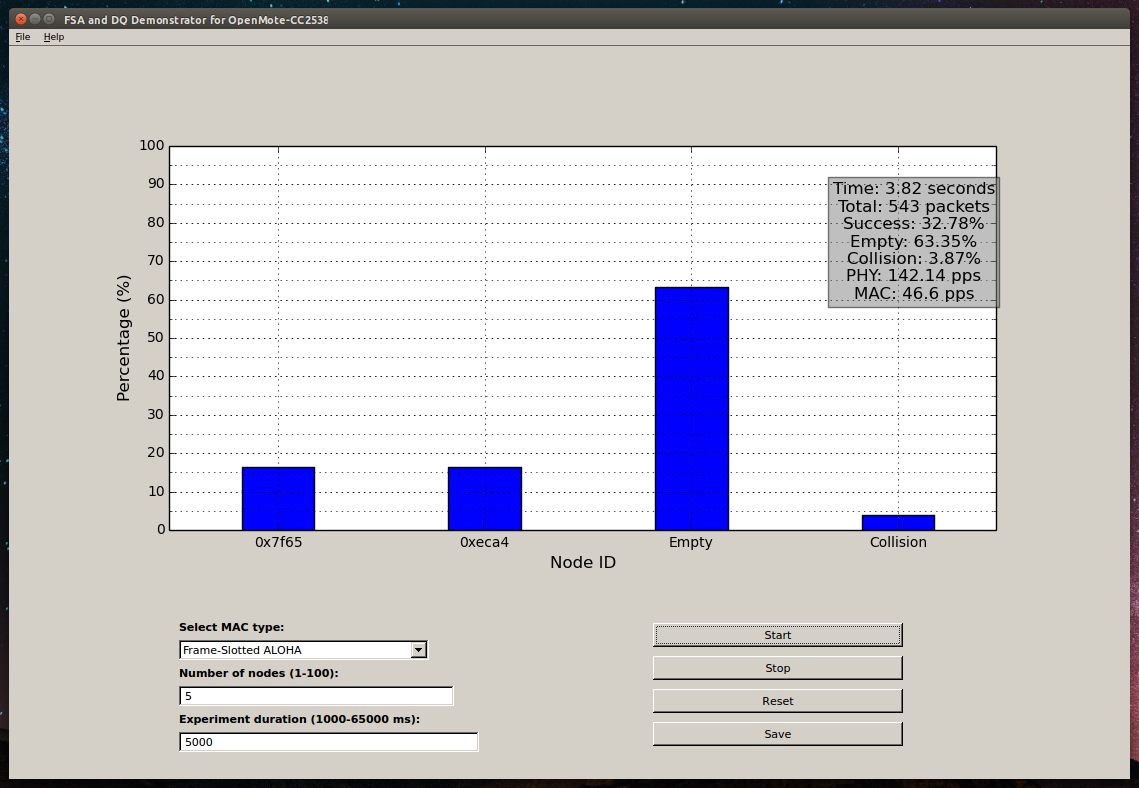
\includegraphics[width=0.75\linewidth]{07-fsa-k5n2}
    \caption{FSA results with $k=5$, $n=2$.}
    \label{fig:07-fsa-k5n2}
\end{figure}

In the fifth experiment, the number of contending nodes is the same but the number of slots per frame increases to ten ($k=10$, $n=2$). According to the formula presented earlier, under such conditions the success probability of each individual node should be $9\%$ and the overall success probability should be $18\%$. As depicted in Figure~\ref{fig:07-fsa-k10n2}, the individual node success probability is around $9\%$ and the overall success probability is $16.82\%$. Again, the obtained results are in accordance with the theoretical results because the capture effect does not play a significant role in the overall results.

% FSA results with k=10, n=2
\begin{figure}[!ht]
    \centering
	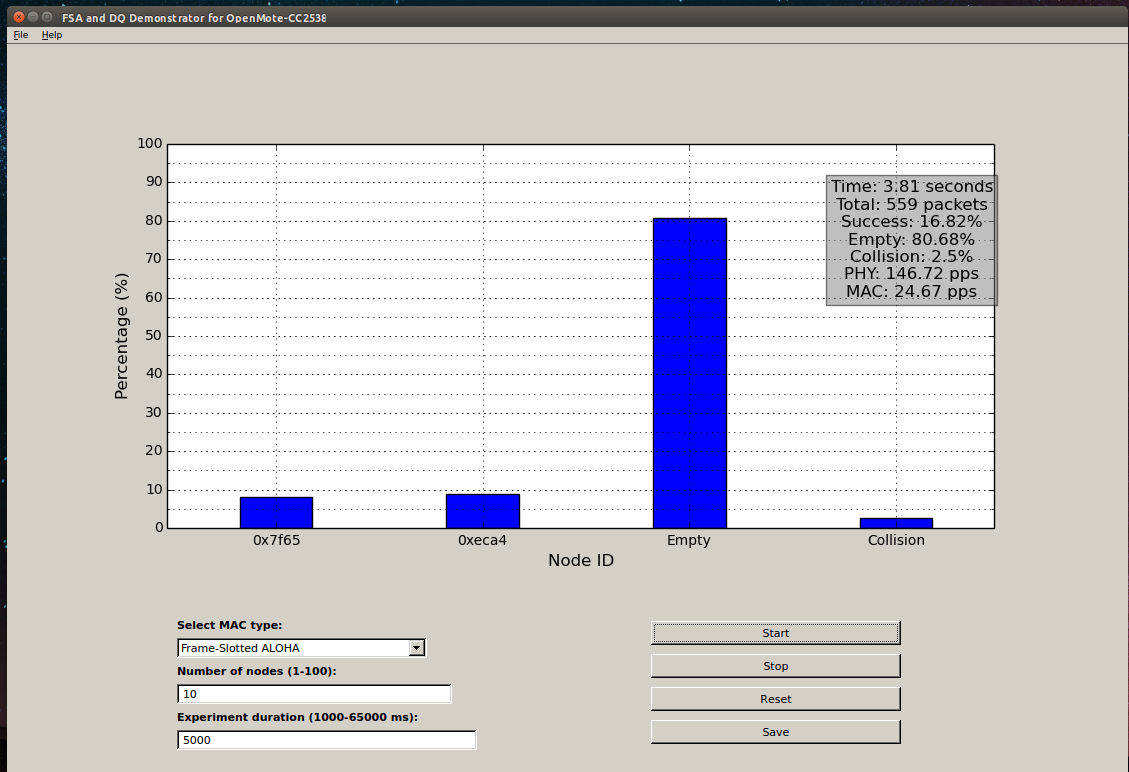
\includegraphics[width=0.75\linewidth]{07-fsa-k10n2}
    \caption{FSA results with $k=10$, $n=2$.}
    \label{fig:07-fsa-k10n2}
\end{figure}

Finally, in the sixth experiment the number of nodes is equal to the number of contending nodes ($k=5$, $n=5$). According to the formula presented earlier, under such conditions the success probability of each individual node should be $8.2\%$ and the overall success probability should be $41\%$. As depicted in figure~\ref{fig:07-fsa-k5n5}, the obtained overall success probability is above the theoretical value ($61.33\%$) and it is also possible to observe that certain nodes are also capable to transmit its data packets with a success probability higher than the expected value ($>10\%$). In contrast with the previous experiments, when the number of slots per frame is equal to the number of contending nodes the influence of the capture effect plays an important role.

% FSA results with k=5, n=5
\begin{figure}[!ht]
    \centering
	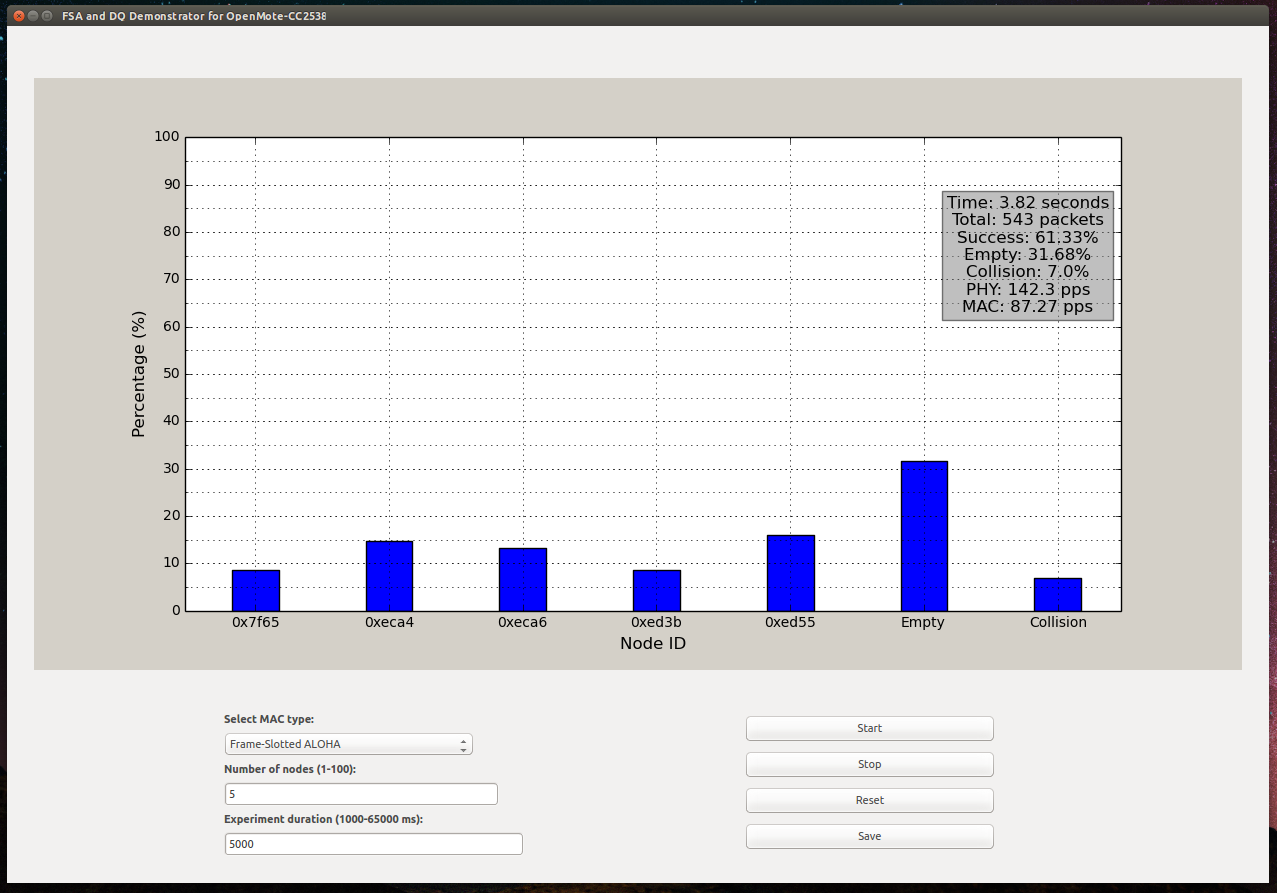
\includegraphics[width=0.75\linewidth]{07-fsa-k5n5}
    \caption{FSA results with $k=5$, $n=5$.}
    \label{fig:07-fsa-k5n5}
\end{figure}

%%
% Distributed Queuing
%%
\section{Distributed Queuing}
Contrarily to FSA, the performance of DQ is independent of the number of nodes that are present in the network. Such behaviour is due to the fact that the process to transmit data packets is split into two sub-periods which are decoupled from each other and are interleaved in time. Nodes first need to transmit an ARP (Access Request Packet) in the access sub-period to obtain access to the network. If the transmission of the ARP results in a collision with other nodes, these nodes join the CRQ (Collision Resolution Queue) to resolve such collision. The collision is resolved by repeating the process of transmitting an ARP in the access sub-period when the nodes are at the head of the CRQ. Once the collision is resolved the nodes that have solved the collision are allowed to join the DTQ (Data Transmit Queue). The nodes then need to wait until they are at the head of the DTQ to transmit their data packets in the data transmission sub-period.

The process to transmit ARP packets in the access sub-period and to join the network and to transmit a data packet in the data transmission sub-period is governed by a set of rules. For example, in order to transmit an ARP packet to join the network the CRQ must be empty, that is, the CRQ is blocking. Moreover, the collision resolution mechanism implemented in the CRQ is based on a split tree algorithm, which ensures that collisions are resolved in logarithmic time regardless of the distribution of collisions. Similarly, access to the DTQ is exclusive in the sense that a given node can only hold one position in the DTQ and that each position in the DTQ can only be hold by one node. This ensures that there are no collisions during the transmission of data packets in the data transmission sub-period which, in turn, ensures that the overall network performance is always close to the theoretical maximum regardless of the number of nodes.

Given the operation of DQ, in the following paragraphs its performance is demonstrated with various number of contending nodes present in each configuration. The first experiment is with only one node in the network ($n=1$). Since a node needs to transmit an ARP in the access sub-period and then wait until the next data transmission sub-period to transmit its data packet, the success probability of the node is expected to be $50\%$. In turn, since there is only one node in the network the empty probability is also $50\%$. As it can be seen in Figure~\ref{fig:07-dq-n1}, the success probability of the node is $50\%$ and the empty probability of the network is $50\%$, which is in accordance with the expected results.

% DQ results with n=1
\begin{figure}[!ht]
    \centering
	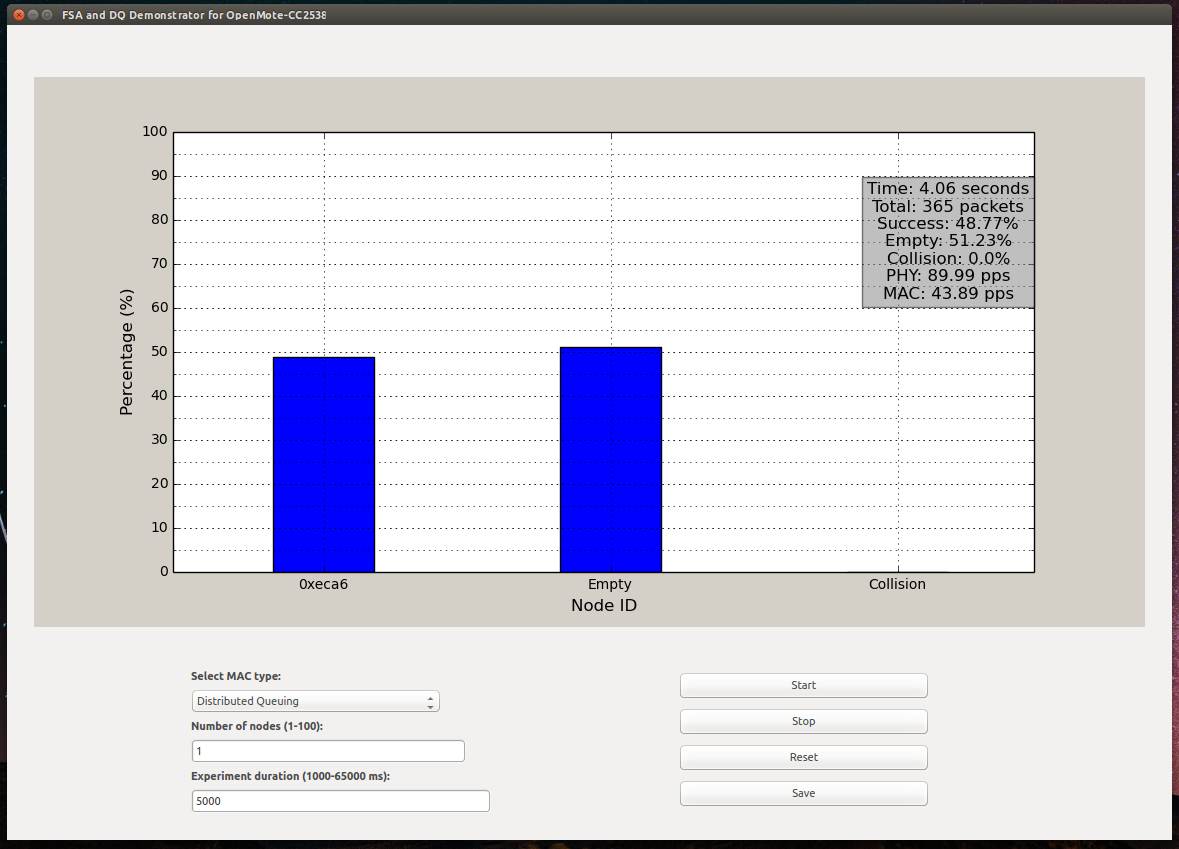
\includegraphics[width=0.75\linewidth]{07-dq-n1}
    \caption{DQ results with $n=1$.}
    \label{fig:07-dq-n1}
\end{figure}

The second experiment is with five nodes in the network ($n=5$). Under such scenario, the success probability for each node is expected to be around $20\%$ and the success probability of the whole network is expected to be close to $100\%$. As depicted in Figure~\ref{fig:07-dq-n5}, the success probability of each node is close to $20\%$ and the success probability of the whole network is $98.36\%$, which is in accordance with the expected results. The empty percentage of the whole network ($1.64\%$) is related to the number of periods that it takes to initially resolve the collisions among the five nodes and start transmitting data packets.

% DQ results with n=5
\begin{figure}[!ht]
    \centering
	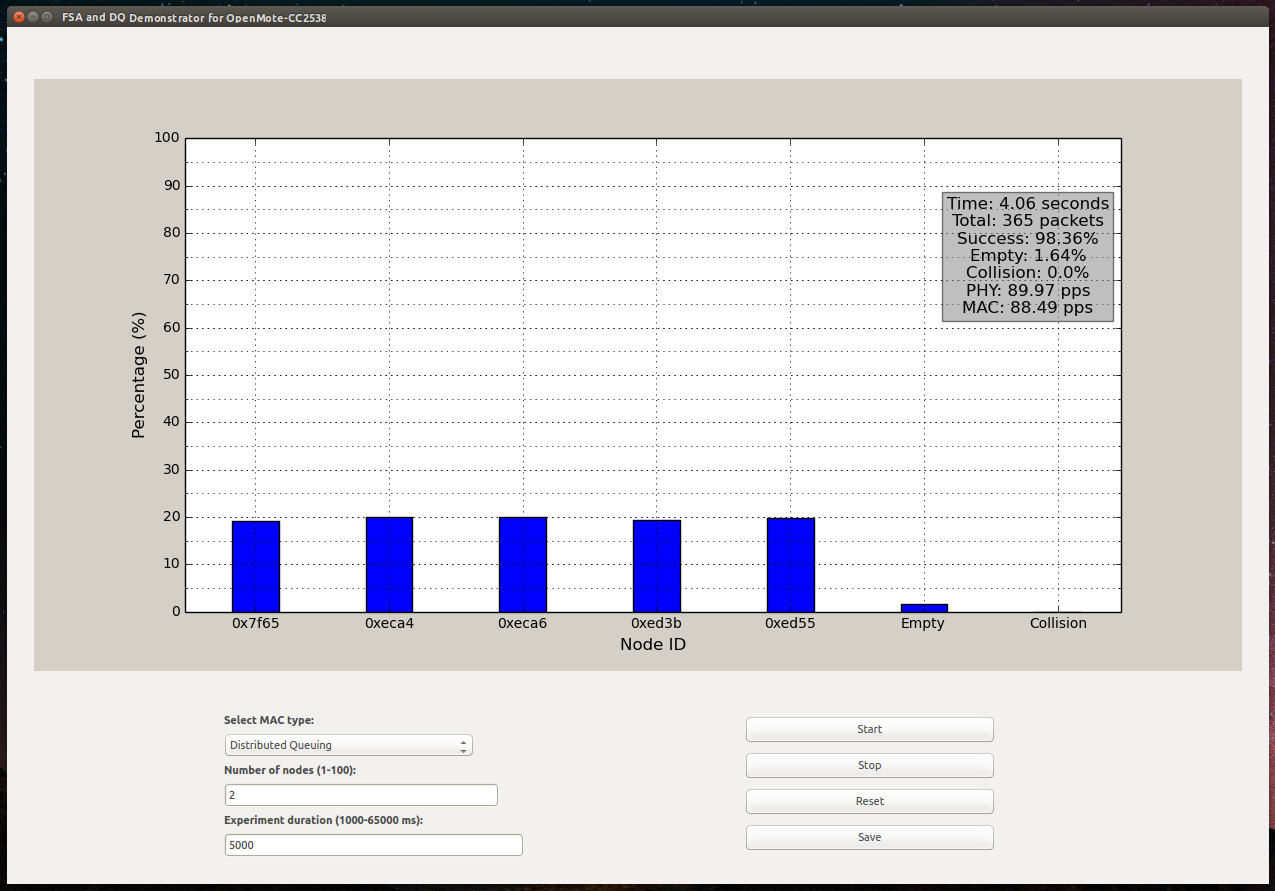
\includegraphics[width=0.75\linewidth]{07-dq-n5}
    \caption{DQ results with $n=5$.}
    \label{fig:07-dq-n5}
\end{figure}

Finally, the third experiment is with ten nodes in the network ($k=10$). Under such scenario, the success probability for each node is expected to be around $10\%$ and the success probability of the whole network is expected to be close to $100\%$. As depicted in Figure~\ref{fig:07-dq-n10}, the success probability of each node is close to $10\%$ and the success probability of the whole network is $99.18\%$, which is in accordance with the expected results. Again, the empty probability of the network ($0.82\%$) is related to the number of periods that it takes to initially resolve the collisions among the ten nodes and start transmitting data packets.

% DQ results with n=10
\begin{figure}[!ht]
    \centering
	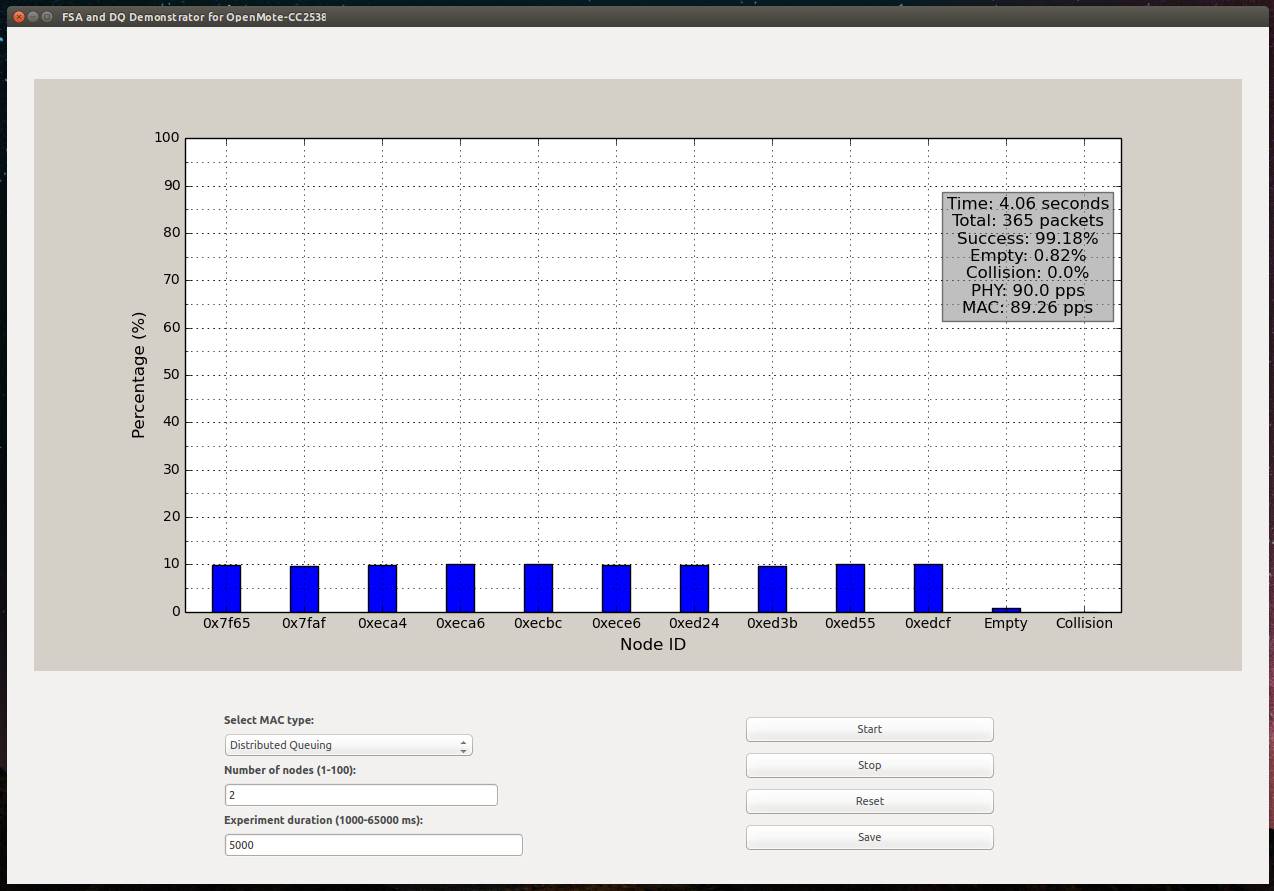
\includegraphics[width=0.75\linewidth]{07-dq-n10}
    \caption{DQ results with $n=10$.}
    \label{fig:07-dq-n10}
\end{figure}

Last but not least, it is important to remark that the capture effect does not affect the performance of DQ regardless the number of nodes that are present in the network, as demonstrated in the second and third experiments. The rationale behind such fact is that the application of the rules to manage the CRQ and DTQ queues decouples the performance of the data-link layer from performance of the physical layer. That is, even the capture effect takes place at the physical layer, the data-link layer performance is decoupled from its effects because the CRQ is blocking and the DTQ ensures that there are no collisions in the transmission of data packets. In contrast to FSA, this represents an important benefit in scenarios where nodes are operated using batteries because all nodes will be depleted at the same rate regardless of their relative position to the gateway.